\documentclass[11pt,landscape,a4paper]{article}
\usepackage[utf8]{inputenc}
\usepackage[T1]{fontenc}
%\usepackage[LY1,T1]{fontenc}
%\usepackage{frutigernext}
%\usepackage[lf,minionint]{MinionPro}
\usepackage{tikz}
\usetikzlibrary{shapes,positioning,arrows,fit,calc,graphs,graphs.standard}
\usepackage[nosf]{kpfonts}
\usepackage[t1]{sourcesanspro}
\usepackage{multicol}
\usepackage{wrapfig}
\usepackage[top=4mm,bottom=4mm,left=4mm,right=4mm]{geometry}
\usepackage[framemethod=tikz]{mdframed}
\usepackage{microtype}
\usepackage{pdfpages}
\usepackage[shortlabels]{enumitem}
\usepackage{flushend}
\usepackage[abbreviations]{foreign}
\usepackage{tcolorbox}
\usepackage{amsthm}
\usepackage{caption}


\raggedend 

\newif\iflong
\longtrue % \longfalse for short version and \longtrue for long version
\newcommand{\inLongVersion}[1]{\iflong #1\fi}


\setlist{nosep}
\setlist[itemize]{leftmargin=*}
\setlist[enumerate]{leftmargin=*}

\newcommand{\score}{\text{score}}
\newcommand{\encoder}{\text{encoder}}
\newcommand{\decoder}{\text{decoder}}
\newcommand{\E}{\mathbb{E}}
\newcommand{\Dist}{\mathcal{D}}
\newcommand{\normal}{\mathcal{N}}
\newcommand{\prob}{\mathbb{P}}
\newcommand{\HEADER}[1]{\begin{tcolorbox}
    \centering
    #1
\end{tcolorbox}}

\DeclareMathOperator{\cov}{\textbf{Cov}}
\DeclareMathOperator{\var}{\textbf{Var}}
\DeclareMathOperator{\argmin}{\textbf{argmin}}
\DeclareMathOperator{\argmax}{\textbf{argmax}}
\DeclareMathOperator{\sgn}{\textbf{sgn}}
\DeclareMathOperator{\dir}{\textbf{Dir}}
\DeclareMathOperator{\cat}{\textbf{Cat}}
\DeclareMathOperator{\vol}{\textbf{vol}}
\DeclareMathOperator{\nnz}{\textbf{nnz}}
\DeclareMathOperator{\Tr}{\textbf{Tr}}
\DeclareMathOperator{\im}{\textbf{im}}
\DeclareMathOperator{\val}{\textbf{val}}






\let\bar\overline

\definecolor{myblue}{cmyk}{0,0,0,1}


\def\firstcircle{(0,0) circle (1.5cm)}
\def\secondcircle{(0:2cm) circle (1.5cm)}

\colorlet{circle edge}{myblue}
\colorlet{circle area}{myblue!5}

\tikzset{filled/.style={fill=circle area, draw=circle edge, thick},
    outline/.style={draw=circle edge, thick}}
    
\pgfdeclarelayer{background}
\pgfsetlayers{background,main}

\everymath\expandafter{\the\everymath \color{myblue}}
\everydisplay\expandafter{\the\everydisplay \color{myblue}}

\renewcommand{\baselinestretch}{.8}
\pagestyle{empty}

\global\mdfdefinestyle{header}{%
linecolor=gray,linewidth=1pt,%
leftmargin=0mm,rightmargin=0mm,skipbelow=0mm,skipabove=0mm,
}

\newcommand{\header}{
\begin{mdframed}[style=header]
\footnotesize
\sffamily
\centering
AML, Yuhao Mao,~Page~\thepage
\end{mdframed}
}

\makeatletter % Author: https://tex.stackexchange.com/questions/218587/how-to-set-one-header-for-each-page-using-multicols
\renewcommand{\section}{\@startsection{section}{1}{0mm}%
                                {.5ex}%
                                {.5ex}%x
                                {\color{myblue}\sffamily\bfseries}}
\renewcommand{\subsection}{\@startsection{subsection}{2}{0mm}%
                                {.2ex}%
                                {.2ex}%x
                                {\sffamily\bfseries}}
\renewcommand{\subsubsection}{\@startsection{subsubsection}{3}{0mm}%
                                {.1ex}%
                                {.1ex}%x
                                {\sffamily\itshape}}



\def\multi@column@out{%
   \ifnum\outputpenalty <-\@M
   \speci@ls \else
   \ifvoid\colbreak@box\else
     \mult@info\@ne{Re-adding forced
               break(s) for splitting}%
     \setbox\@cclv\vbox{%
        \unvbox\colbreak@box
        \penalty-\@Mv\unvbox\@cclv}%
   \fi
   \splittopskip\topskip
   \splitmaxdepth\maxdepth
   \dimen@\@colroom
   \divide\skip\footins\col@number
   \ifvoid\footins \else
      \leave@mult@footins
   \fi
   \let\ifshr@kingsaved\ifshr@king
   \ifvbox \@kludgeins
     \advance \dimen@ -\ht\@kludgeins
     \ifdim \wd\@kludgeins>\z@
        \shr@nkingtrue
     \fi
   \fi
   \process@cols\mult@gfirstbox{%
%%%%% START CHANGE
% \ifnum\count@=\numexpr\mult@rightbox+2\relax
%           \setbox\count@\vsplit\@cclv to \dimexpr \dimen@-1cm\relax
% \setbox\count@\vbox to \dimen@{\vbox to 1cm{\header}\unvbox\count@\vss}%
% \else
%       \setbox\count@\vsplit\@cclv to \dimen@
% \fi
\setbox\count@\vsplit\@cclv to \dimen@
%%%%% END CHANGE
            \set@keptmarks
            \setbox\count@
                 \vbox to\dimen@
                  {\unvbox\count@
                   \remove@discardable@items
                   \ifshr@nking\vfill\fi}%
           }%
   \setbox\mult@rightbox
       \vsplit\@cclv to\dimen@
   \set@keptmarks
   \setbox\mult@rightbox\vbox to\dimen@
          {\unvbox\mult@rightbox
           \remove@discardable@items
           \ifshr@nking\vfill\fi}%
   \let\ifshr@king\ifshr@kingsaved
   \ifvoid\@cclv \else
       \unvbox\@cclv
       \ifnum\outputpenalty=\@M
       \else
          \penalty\outputpenalty
       \fi
       \ifvoid\footins\else
         \PackageWarning{multicol}%
          {I moved some lines to
           the next page.\MessageBreak
           Footnotes on page
           \thepage\space might be wrong}%
       \fi
       \ifnum \c@tracingmulticols>\thr@@
                    \hrule\allowbreak \fi
   \fi
   \ifx\@empty\kept@firstmark
      \let\firstmark\kept@topmark
      \let\botmark\kept@topmark
   \else
      \let\firstmark\kept@firstmark
      \let\botmark\kept@botmark
   \fi
   \let\topmark\kept@topmark
   \mult@info\tw@
        {Use kept top mark:\MessageBreak
          \meaning\kept@topmark
         \MessageBreak
         Use kept first mark:\MessageBreak
          \meaning\kept@firstmark
        \MessageBreak
         Use kept bot mark:\MessageBreak
          \meaning\kept@botmark
        \MessageBreak
         Produce first mark:\MessageBreak
          \meaning\firstmark
        \MessageBreak
        Produce bot mark:\MessageBreak
          \meaning\botmark
         \@gobbletwo}%
   \setbox\@cclv\vbox{\unvbox\partial@page
                      \page@sofar}%
   \@makecol\@outputpage
     \global\let\kept@topmark\botmark
     \global\let\kept@firstmark\@empty
     \global\let\kept@botmark\@empty
     \mult@info\tw@
        {(Re)Init top mark:\MessageBreak
         \meaning\kept@topmark
         \@gobbletwo}%
   \global\@colroom\@colht
   \global \@mparbottom \z@
   \process@deferreds
   \@whilesw\if@fcolmade\fi{\@outputpage
      \global\@colroom\@colht
      \process@deferreds}%
   \mult@info\@ne
     {Colroom:\MessageBreak
      \the\@colht\space
              after float space removed
              = \the\@colroom \@gobble}%
    \set@mult@vsize \global
  \fi}

\makeatother
\setlength{\parindent}{0pt}




\begin{document}
%\footnotesize
\small
\begin{multicols*}{3}

% Part 1: Convex Optimization

\HEADER{Convex Optimization}

% Part 2: spectral graph theory
\section{Convex Functions}

Definition:
\begin{enumerate}
    \item  A set $S \subseteq \mathbb{R}^{n}$ is called a convex set if any two points in $S$ contain their line, i.e. for any $\boldsymbol{x}, \boldsymbol{y} \in S$ we have that $\theta \boldsymbol{x}+(1-\theta) \boldsymbol{y} \in S$ for any $\theta \in[0,1]$.
    \item For a convex set $S \subseteq \mathbb{R}^{n}$, we say that a function $f: S \rightarrow \mathbb{R}$ is convex on $S$ if for any two points $\boldsymbol{x}, \boldsymbol{y} \in S$ and any $\theta \in[0,1]$ we have that
    $
    f(\theta \boldsymbol{x}+(1-\theta) \boldsymbol{y}) \leq \theta f(\boldsymbol{x})+(1-\theta) f(\boldsymbol{y}).
    $
\end{enumerate}

Properties:
\begin{enumerate}
    \item If $f$ is convex, then all its sub-levels $\{x: f(x)\le \alpha\}$ is convex. The reverse is not true, \eg, $x^3$.
\end{enumerate}

\subsection{First-order Characterization}
\textbf{Theorem}:
Let $S$ be an open convex subset of $\mathbb{R}^{n}$, and let $f: S \rightarrow \mathbb{R}$ be a differentiable function. Then, $f$ is convex if and only if for any $\boldsymbol{x}, \boldsymbol{y} \in S$ we have that $f(\boldsymbol{y}) \geq f(\boldsymbol{x})+$ $\boldsymbol{\nabla} f(\boldsymbol{x})^{\top}(\boldsymbol{y}-\boldsymbol{x}) .$

\subsection{Second-order Characterization}
\textbf{Theorem}:
Let $S \subseteq \mathbb{R}^{n}$ be open and convex, and let $f: S \rightarrow \mathbb{R}$ be twice continuously differentiable.
\begin{enumerate}
    \item $H_{f}(\boldsymbol{x})$ is positive semi-definite for any $\boldsymbol{x} \in S$ $\Leftrightarrow$ $f$ is convex on $S$.
    \item If $H_{f}(\boldsymbol{x})$ is positive definite for any $\boldsymbol{x} \in S$ then $f$ is strictly convex on $S$. The opposite is not true, \eg, for $f(x)=x^4$ at $x=0$.
\end{enumerate}


\HEADER{Spectral Graph Theory}

\emph{This part is organized as follows: the first two sections discuss graph Laplacian in the spectral domain, by bounding its eigenvalues and introducing its importance (Cheeger's inequality). The random walk section provides a use case of graph spectral in the analysis of convergence, and introduces the importance of Laplacian linear equations. The next two sections show how to solve it exactly by applying pseudo inverse, as the Laplacian is non-invertible. The rest sections show how to approximate a graph Laplacian and solve the Laplacian linear equation approximately and more efficiently.}

\section{Spectral Domain of the Graph}

We assume the graph has $n$ vertices and $m$ edges. The vertex set is $V$ and the edge set is $E$.

\subsection{Graph Laplacian}

Define $D:= \diag_{v \in V} d(v)$ be the degree (sum of all weights of the edges incident to $v$) matrix, and $A$ be the adjacency matrix. Then the graph Laplacian $L$ is defined to be $L:=D-A$. For electrical graphs, $L=BR^{-1}B^\top$, where $B$ of shape $(n, m)$ is the vertex-edge incidence matrix (-1 for one end and 1 for another end), and $R:=\diag_{e \in E} 1/r_e$.

Properties:
\begin{enumerate}
    \item Given voltage vector $x$ of shape $(n, 1)$, $x^\top L x = \sum_{(u,v) \in E} \frac{(x(u)-x(v))^2}{r(u,v)}$.
    \item $L$ is positive semi-definite, and the dimension of $\ker(L)$ is equal to the number of connected components in the graph $G$. $\ker(L)$ is spanned by $\boldsymbol{1}_{V_i}$, where $V_i$ is the vertices of the connected components.
\end{enumerate}

\subsection{Courant-Fischer Theorem}
\begin{enumerate}
    \item \textbf{Eigenvalue version}: Let $A$ be a symmetric matrix with eigenvalues $\lambda_1 \le \dots \le \lambda_n$, then 
    $$\lambda_{i}=\min _{\substack{\text { subspace } W \subseteq \mathbb{R}^{n} \\ \operatorname{dim}(W)=i}} \max _{\substack{x \in W \\ x \neq \mathbf{0}}} \frac{x^{\top} A x}{x^{\top} x} = \max _{\substack{\text { subspace } W \subseteq \mathbb{R}^{n} \\ \operatorname{dim}(W)=n+1-i}} \min _{\substack{x \in W\\ x \neq \mathbf{0}}} \frac{x^{\top} A x}{x^{\top} x}.$$
    \item \textbf{Eigenbasis version}: Let $A$ be a symmetric matrix with eigenvalues $\lambda_1 \le \dots \le \lambda_n$ and corresponding orthonormal eigenvectors $x_1, \dots, x_n$, then
    $$\lambda_{i}=\min _{\substack{x \perp x_{1}, \ldots x_{i-1} \\ x \neq \mathbf{0}}} \frac{x^{\top} A x}{x^{\top} x} = \max _{\substack{x \perp x_{i+1}, \ldots x_{n} \\ x \neq \mathbf{0}}} \frac{x^{\top} A x}{x^{\top} x}.$$
\end{enumerate}
Note that we also have $\lambda_i = \frac{x_i^\top A x_i}{x_i^\top x_i}$.

Applying Courant-Fischer theorem, we have $\lambda_2 x^\top x  \le x^\top L x \le \lambda_n x^\top x$ for all $x \perp \boldsymbol{1}$, as $\boldsymbol{1}$ is the eigenvector of $L$ corresponding to eigenvalue $0$. For connected graphs, $\lambda_2 > 0$.

\subsection{PSD Order (Loewner Order)}

Defined only for symmetric matrices: $A \preceq B$ iff for all $x \in \mathbb{R}^{n}$, we have $x^{\top} A x \leq x^{\top} B x$. We also define $G \preceq H$ for two graphs $G$ and $H$ iff $L_G \preceq L_H$. We always have $G \succeq H$ if $H$ is a subgraph of $G$.

Properties:
\begin{enumerate}
    \item If $A \preceq B$ and $B \preceq C$, then $A \preceq C$.
    \item If $A \preceq B$, then $A+C \preceq B+C$ for any symmetric $C$.
    \item If $A \preceq B$ and $C \preceq D$, then $A+C \preceq B+D$.
    \item If $A \succ 0$ and $\alpha \ge 1$, then $\frac{1}{\alpha} A \preceq A \preceq \alpha A$.
    \item If $A \preceq B$, then $\lambda_i(A) \le \lambda_i(B)$ for all $i$. Proof by Courant-Fischer theorem. The converse is not true.
    \item For any matrix $C$, if $A \preceq B$, then $C^\top A C \preceq C^\top B C$.
    \item If $0 \preceq A \preceq B$, then $B^{-1} \preceq A^{-1}$.
\end{enumerate}

\subsection{Bounding the $\lambda_2$ and $\lambda_n$}

\subsubsection{Test Vector Method}
Since $\lambda_2 \le \frac{y^\top L y}{y^\top y}$ for any $y \perp \boldsymbol{1}$, we can upper bound the $\lambda_2$ by any \textbf{test vector} $y$. Similarly, we can lower bound the $\lambda_n$ by test vectors by $\lambda_n \ge \frac{y^\top L y}{y^\top y}$.

\begin{enumerate}
    \item For a complete graph $K_n$, $L = n \boldsymbol{I} - \boldsymbol{1}\boldsymbol{1}^\top$ and for any $x \perp \boldsymbol{1}$ we have $x^\top L x = n x^\top x$. Therefore, $\lambda_2(K_n) = \dots = \lambda_n(K_n) = n$ and any $x \perp \boldsymbol{1}$ is an eigenvector.
    \item For a path graph $P_n$, let $x(i) = n+1 - 2i$ be the test vector which satisfies $x \perp \boldsymbol{1}$, we get $\lambda_2(P_n) \le \frac{12}{n^2}$. Let $x(1)=-1$, $x(n)=1$ and $x(i)=0$ for other $i$ to be the test vector, we get $\lambda_n(P_n) \ge 1$.
    \item For a complete binary tree $T_n$ (depth equals zero for a single root), let $x(i)=0$ for all non-leaf nodes, $x(i)=-1$ for even-numbered leaf nodes and $x(i)=1$ for odd-numbered leaf nodes be the test vector, we get $\lambda_n(T_n) \ge 1$. Let $x(1)=0$, $x(i)=1$ for the left subtree of the root and $x(i)=-1$ for the right subtree of the root be the test vector, we get $\lambda_2(T_n) \le \frac{2}{n-1}$.
\end{enumerate}

\subsubsection{Consequences of PSD Order}

Since $x^\top (D-A) x = \sum_{(u,v)} w(u,v)(x(u)-x(v))^2 \ge 0$ and $x^\top (D+A) x = \sum_{(u,v)} w(u,v)(x(u)+x(v))^2 \ge 0$, we have $D \succeq A$ and $D \succeq -A$. In addition, we have $D \preceq (\max D_{i,i}) \boldsymbol{I}$. Therefore, we have $L = D-A \preceq 2D \preceq (2\max D_{i,i}) \boldsymbol{I}$, which implies $\lambda_n \le 2\max D_{i,i}$ for any graph. For unit-weight graphs, this means $\lambda_n \le 2 \max \text{degree}(v)$. The bound is tight for a single-edge graph.

To get lower bounds of $\lambda_2(H)$, we first establish $f(n) H \succeq G$ for some $G$ with known lower bounds on $\lambda_2(G)$. Usually $G=K_n$ because $\lambda_2(K_n) = n$. Then it follows that $\lambda_2(H) \ge \lambda_2(G)/f(n)$.

\begin{enumerate}

    \item \textbf{Path Graph $P_n$}: Let $G_{i,j}$ denote a unit-weight graph consisting of one edge $(i,j)$ and $P_n$ be the path graph connecting $1$ and $n$. Then $(n-1)P_n \succeq G_{1,n}$. Proof follows from applying Cauchy-Schwartz for $\delta_i:=x(i+1)-x(i)$. For weighted paths, we have $G_{1, n} \preceq\left(\sum_{i=1}^{n-1} \frac{1}{w_{i}}\right) \sum_{i=1}^{n-1} w_{i} G_{i, i+1}$.

    Applying path inequality, we have $K_n = \sum_{i<j} G_{i,j} \preceq \sum_{i<j} (j-i) P_{i,j} \preceq \sum_{i<j} (j-i) P_n \preceq n^3 P_n$, which implies $\lambda_2(P_n) \ge \lambda_2(K_n)/n^3 = 1/n^2$.



    \item \textbf{Any unit-weight graph $G$}: Define the diameter $D$ of a graph $G$ to be the maximum length of the shortest paths between any two nodes. Let $G^s_{i,j}$ be the shortest path from $i$ to $j$. Applying path inequality, we have $K_n = \sum_{i<j} G_{i,j} \preceq \sum_{i<j} D G^s_{i,j} \preceq \sum_{i<j} DG \preceq n^2 DG$, which implies $\lambda_2(G) \ge \frac{1}{nD}$.

    \item \textbf{Complete Binary Tree $T_n$}: Define $G_e$ be the single-edge graph with edge $e$, and $T_{i,j}$ be the unique path between $i$ and $j$. Applying the weighted path inequality, we have $K_n = \sum_{i<j} G_{i,j} \preceq \sum_{i<j}\left(\left(\sum_{e \in T^{i, j}} \frac{1}{w(e)}\right)\left(\sum_{e \in T^{i, j}} w(e) G_{e}\right)\right) \preceq\left(\max _{i<j} \sum_{e \in T^{i, j}} \frac{1}{w(e)}\right)\left(\sum_{i<j} \sum_{e \in T^{i, j}} w(e) G_{e}\right)$. For $e$ connecting level $i$ and $i+1$ for $i \in [d-1]$, we set $w(e)=2^i$. Then $\max _{i<j} \sum_{e \in T^{i, j}} \frac{1}{w(e)} \le 4$. Since the number of occurrence of $e$ in $T^{i,j}$ for any $i<j$ is upper bounded by $n^2 2^{-i}$, we have $\sum_{i<j} \sum_{e \in T^{i, j}} w(e) G_{e} \preceq \sum_{e} w(e) n^2 2^{-i} G_e = \sum_e n^2 G_e = n^2T_n$. Therefore, $K_n \preceq 4n^2T_n$, which implies $\lambda_2(T_n) \ge \frac{1}{4n}$.
    
\end{enumerate}




\section{Conductance}

Definitions:
\begin{enumerate}
    \item \textbf{Conductance of a vertex subset}: Given $\emptyset \subset S \subset V$, the conductance $\phi(S) := \phi(S)=\frac{|E(S, V \backslash S)|}{\min \{\vol(S), \vol(V \backslash S)\}}$, where $\vol(S) := \sum_{v \in S} \text{degree}(v)$. Define $\boldsymbol{1}_S$ to be the $n$-dimensional vector with only 1 for the vertices of $S$ and 0 for the vertices of $V \setminus S$. Assuming $\vol(S) \le \vol(V)/2$, thus $|E(V, V\setminus S)|= \sum_{(u,v)\in E} (\boldsymbol{1}_S(u) - \boldsymbol{1}_S(v))^2 = \boldsymbol{1}_S^\top L \boldsymbol{1}_S$ and $\vol(S) = \boldsymbol{1}_S^\top D \boldsymbol{1}_S$. Then $\phi(S) = \frac{\boldsymbol{1}_S^\top L \boldsymbol{1}_S}{\boldsymbol{1}_S^\top D \boldsymbol{1}_S}$.

    \item \textbf{Conductance of a graph}: The conductance $\phi(G) := \min_{\emptyset \subset S \subset V} \phi(S) = \min_{\substack{\emptyset \subset S \subset V \\ \vol(S)\le\vol(V)/2}} \phi(S).$

    \item \textbf{$\phi$-expander}: For any $\phi \in (0,1]$, we call a graph $G$ to be a $\phi$-expander if $\phi(G)\ge \phi$.
    \item \textbf{$\phi$-expander decomposition of quality $q$}: A partition $\{X_i\}$ of the vertex set $V$ is called a $\phi$-expander decomposition of quality $q$ if (1) each induced graph $G[X_i]$ is a $\phi$-expander, and (2.i) \#edges not contained in any $G[X_i]$ is at most $q\cdot\phi\cdot m$. The second condition is equivalent to (2.ii) The partition removes at most $q\cdot\phi\cdot m$ edges.
    \item \textbf{Normalized Laplacian}: We define the \textit{normalized Laplacian} to be $N := D^{-1/2} L D^{-1/2}$. $N$ is still PSD, with first eigenvalue equals 0 associated with eigenvector $D^{1/2}\boldsymbol{1}$. By Courant-Fischer theorem, $\lambda_2(N) = \min_{x \perp D^{1/2}\boldsymbol{1}} \frac{x^\top N x}{x^\top x} = \min_{z \perp d} \frac{z^\top L z}{z^\top D z}$.
\end{enumerate}

\subsection{Cheeger's Inequality}

Notice that the $\lambda_2(N)$ has similar forms to $\phi(G)$. Cheeger's inequality aims to bound $\phi(G)$ by $\lambda_2(N)$.

\textbf{Cheeger's Inequality}: $\frac{\lambda_2(N)}{2} \le \phi(G) \le \sqrt{2\lambda_2(N)}$.

The lower bound is proved by restricting the minimum in $\lambda_2(N)$ to be $z_S = \boldsymbol{1}_S - \alpha \boldsymbol{1}$ for some $\alpha$ such that $z_S \perp d$. The upper bound is proved by constructing $S$ for any $z \perp d$ such that $\frac{\boldsymbol{1}_S^\top L \boldsymbol{1}_S}{\boldsymbol{1}_S^\top D \boldsymbol{1}_S} \le \sqrt{2 \frac{z^\top L z}{z^\top D z}}$.



\section{Random Walk}

\section{Pseudo-Inverse and Effective Resistance}

Given a Laplacian $L$, its (Moore-Penrose) pseudo inverse is defined to be either of the two equivalents:
\begin{enumerate}
    \item A matrix $L^+$ that is (1) symmetric, (2) $L^+ v=0$ for $v \in \ker(L)$, and (3) $L^+ L v = L L^+ v = v$ for  $v \in \ker(L)$.
    \item Let $\lambda_i, v_i$ be the $i$-th eigenvalue and eigenvector. Then $L^+ = \sum_{\lambda_i \ne 0} \lambda_i^{-1} v_i v_i^\top$.
\end{enumerate}

Property:
\begin{itemize}
    \item Assume $M=X Y X^\top$, where $X$ is real and invertible, and $Y$ is real and symmetric. Let $\Pi_M$ be the orthogonal projection to the image of $M$. Then $M^+ = \Pi_M (X^\top)^{-1} Y^+ X^{-1} \Pi_M$.
    \item For symmetric $L$, $\Pi_L:= \sum_{\lambda_i \ne 0} v_i v_i^\top =  L^{+/2} L L^{+/2} = L^+ L = L L^+$ is the orthogonal projection to the image of $L$, \ie, $\Pi_L v = 0$ for any $v \in \ker(L)$ and $\Pi_v = v$ for any $v \in \im(L)$. For connected $G$, $\Pi_{L} = \boldsymbol{I} - \frac{1}{n} \boldsymbol{1} \boldsymbol{1}^\top$.
\end{itemize}

The effective resistance between vertex $a$ and $b$ is defined to be the cost (energy lost) to routing one unit (of positive electric charge) from $a$ to $b$: $R_{\text{eff}}(a,b) = \min_{Bf = \boldsymbol{1}_b - \boldsymbol{1}_a} f^\top R f = \tilde{f}^\top R \tilde{f}$, where $\tilde{f}$ is the electric flow. Let $\tilde{x}$ be the electric voltages, we also have $L\tilde{x} = \boldsymbol{1}_b - \boldsymbol{1}_a$, and thus $R_{\text{eff}}(a,b) = \tilde{x}^\top L \tilde{x} = (\boldsymbol{1}_b - \boldsymbol{1}_a)^\top L^+ (\boldsymbol{1}_b - \boldsymbol{1}_a) = \|L^{+/2} (\boldsymbol{1}_b - \boldsymbol{1}_a)\|_2^2$.

Effective Resistance is a distance defined on the vertex pairs, i.e. $R_{\text{eff}}(a,c) \le R_{\text{eff}}(a,b) + R_{\text{eff}}(b,c)$.

\section{Gaussian Elimination for Laplacian}

\subsection{Optimization View}

Solving $Lx = d$ is equivalent to solving $\argmin_x -d^\top x + \frac{1}{2} x^\top L x$. By iteratively optimize over $x_i$, we get a series of similar optimizations. The final optimization is straightforward, then we can back substitute to get $x$.

\subsection{Additive View}

Given an invertible square lower/upper triangular matrix $M$, we can solve $Mx=d$ by back substitution in $O(\nnz(M))$, where $\nnz(M)$ means the number of non-zeros in $M$. Therefore, if we know the \textbf{Cholesky decomposition} $L = M M^\top$ (requires $O(n^3)$), then we can solve $Lx =d = M (M^\top x)$ by (1) solving $M y =d$ then (2) solving $M^\top x =y$ in $O(\nnz(M))$.

However, the Laplacian is non-invertible, leading to one diagonal of $M$ equals 0. Therefore, we need to play a trick. Define $\hat{M}$ equals $M$ but has value 1 for the zero diagonal, and $\hat{D}$ be a diagonal matrix that has value 0 at the zero diagonal of $M$ and 1 otherwise. Then $L = \hat{M} \hat{D} \hat{M}^\top$, and each $\hat{M}$ is now invertible. Since $\hat{D}^+ = \hat{D}$, we can find a special solution of $Lx=d$ by (1) solving $\hat{M} z = d$, (2) computing $y = \hat{D} z$, and (3) solving $\hat{M}^\top x = y$. The solution space is obtained by adding a subspace spanned by $\boldsymbol{1}$.

\section{Approximating a Dense Graph in the Spectral Domain}

\subsection{Concentration of Random Matrices}

\begin{enumerate}
    \item \textbf{Chernoff Bound for Bounded independent variables}: Suppose $\{X_i \in \mathbb{R}\}$ are independent random variables and $0\le X_i \le R$. Let $X = \sum_i X_i$ and $\mu = \E X$. Then for any $0<\epsilon \le 1$, we have $\prob(X \ge (1+\epsilon)\mu) \le \exp(-\frac{\epsilon^2 \mu}{4R})$ and $\prob(X \le (1-\epsilon)\mu) \le \exp(-\frac{\epsilon^2 \mu}{4R})$.
    \item \textbf{Bernstein Bound for independent, zero-mean and bounded variables}: Suppose $\{X_i \in \mathbb{R}\}$ are independent, zero-mean random variables and $|X_i| \le R$. Let $X = \sum_i X_i$, and $\sigma^2 = \var(X)$. Then for any $t > 0$, we have $\prob(|X| \ge t) \le 2\exp(\frac{-t^2}{2Rt+4\sigma^2})$.

    The proof is similar to Chernoff bound. (1) $\prob(X\ge t) = \prob(\exp(\theta X) \ge \exp(\theta t)) \le \exp(-\theta t)\E (\exp(\theta X))$, (2) upper bound $\E (\exp(\theta X)) \le \exp(\theta^2 \sigma^2)$ given $\theta \in (0, \frac{1}{R}]$, which allows $\exp(\theta X_i) \le 1+\theta X_i +(\theta X_i)^2$, and (3) take the minimum among $\theta \in (0,\frac{1}{R}]$.

    \item \textbf{Bernstein Bound for independent, zero-mean and bounded symmetric matrices}: Suppose $\{X_i \in \mathbb{R}^{n\times n}\}$ are independent, zero-mean, symmetric random matrices and $\|X_i\| \le R$, where $\|\cdot\|$ is the spectral norm (the largest singular value). Let $X = \sum_i X_i$, and $\sigma^2 = \|\sum_{i=1}^n \E X_i^2\|$. Then $\prob(\|X\|\ge t) \le 2n \exp(\frac{-t^2}{2Rt+4\sigma^2})$.
\end{enumerate}

\subsection{Matrix Functions}

Given a real-valued function $f: \mathbb{R}\rightarrow \mathbb{R}$ and a symmetric matrix $A$ with eigen-decomposition $A=V\Lambda V^\top$, we define $f(A) = V f(\Lambda) V^\top$. This is compatible to the Taylor expansion $f(x) = \sum_i \alpha_i x^i$, as $f(A) = \sum_i \alpha A^i = V (\sum_i \alpha_i f(\Lambda)) V^\top = V f(\Lambda) V^\top$.

\textbf{Monotonicity}: Given $f: \mathcal{D} \rightarrow \mathcal{C}$ and partial orders $\le_{\mathcal{C}}$ and $\le_{\mathcal{D}}$, we call $f$ is monotonically increasing w.r.t. these orders iff for all $d_1 \le_{\mathcal{D}} d_2 \in \mathcal{D}$ we have $f(d_1) \le f(d_2)$. For matrix functions, we use the PSD order as the ordering.

Property:
\begin{itemize}
    \item If the scalar function $f$ is monotonically increasing, then the matrix function $X \rightarrow \Tr(f(X))$ is monotonically increasing.
    \item $\log(\cdot)$ is monotonically increasing.
    \item The matrix function $(\cdot)^2$ and $\exp(\cdot)$ is \textbf{not} monotone.
    \item $\exp(A) \preceq \boldsymbol{I} + A + A^2$ for $\|A\| \le 1$.
    \item $\log(\boldsymbol{I}+A) \preceq A$ for $A \succ -\boldsymbol{I}$.
\end{itemize}

\subsection{Approximating a Dense Graph by Sparse Graphs}

Given PD matrices $A, B$ and $\epsilon>0$, we say $A \approx_{\epsilon} B$ iff $\frac{1}{1+\epsilon} A \preceq B \preceq (1+\epsilon) A$. If $L_G \approx_{\epsilon} L_{\tilde{G}}$ and $|\tilde{E}| \ll |E|$, we call $\tilde{G}$ a spectral sparsifier of $G$.

Properties:
\begin{itemize}
    \item Define $c_G(T) := \sum_{e \in E \cap (T\times V\setminus T)} w(e)$ to be the value of the cut $(T, V\setminus T)$. If $L_G \approx_{\epsilon} L_{\tilde{G}}$, then for all $T \subset V$, we have $\frac{1}{1+\epsilon} c_G(T) \le c_{\tilde{G}}(T) \le (1+\epsilon) c_G(T)$. The proof is by noticing $c_G(T) = 1_T^\top L_G 1_T$.
    \item $L \approx_{\epsilon} \tilde{L} \Leftrightarrow \Pi_L \approx_\epsilon L^{+/2} \tilde{L} L^{+/2}$, as $A \preceq B$ implies $C^\top A C \preceq C^\top B C$ for any $C\in \mathbb{R}^{n\times n}$.
    \item For $\epsilon \le 1$, if $\|\Pi_L - L^{+/2} \tilde{L} L^{+/2}\| \le \epsilon/2$, then $\Pi_L \approx_\epsilon L^{+/2} \tilde{L} L^{+/2}$.
\end{itemize}

Theorem: Consider a connected graph $G=(V, E, w)$, with $n=|V|$. For any $0<\epsilon<1$ and $0<\delta<1$, there exist sampling probabilities $p_{e}$ for each edge $e \in E$ s.t. if we include each edge $e$ in $\tilde{E}$ independently with probabilty $p_{e}$ and set its weight $\tilde{w}(e)=\frac{1}{p_{e}} w(e)$, then with probability at least $1-\delta$ the graph $\tilde{G}=(V, \tilde{E}, \tilde{w})$ satisfies
$
L_{G} \approx_{\epsilon} L_{\tilde{G}} \text { and }|\tilde{E}| \leq O\left(n \epsilon^{-2} \log (n / \delta)\right)
$.
The proof uses Bernstein bounds to prove the concentration of the constructed random graph.

\section{Solving Laplacian Linear Equations Approximately}

Idea: solving Laplacian linear equations requires $O(m)$, which is expensive when the graph is dense. By approximating the Laplacian, we can get an approximation of the solution quickly.

Given PSD matrix $M$ and $d \in \im(M)$, let $M x^* = d$. We say that $\tilde{x}$ is an $\epsilon$-approximate solution to $Mx=d$ iff $\|\tilde{x} - x^*\|_M^2 \le \epsilon \|x^*\|_M^2$, where $\|x\|_M^2 = x^\top M x$. Note that any solution to $M x = d$ has the same $\|\cdot\|_M^2$, as they differ by a vector in the kernel of $M$.

\textbf{Theorem}: Given a Laplacian $\boldsymbol{L}$ of a weighted undirected graph $G=(V, E, \boldsymbol{w})$ with $|E|=m$ and $|V|=n$ and a demand vector $\boldsymbol{d} \in \mathbb{R}^{V}$, we can find $\tilde{\boldsymbol{x}}$ that is an $\epsilon$-approximate solution to $\boldsymbol{L x}=\boldsymbol{d}$, using an algorithm that takes time $O\left(m \log ^{c} n \log (1 / \epsilon)\right)$ for some fixed constant $c$ and succeeds with probability $1-1 / n^{10}$. Note that without known Cholesky decomposition in advance, the exact solution requires $O(n^3)$ and $m \le n^2 / 2$.

% Part 3: Combinatorial Graph Algorithms

\HEADER{Combinatorial Graph Algorithms}

\section{Maximum Flows and Minimum Cuts}

\subsection{Flows}
Definition:
\begin{enumerate}
    \item \textbf{$s$-$t$ flow}: an $s$-$t$ flow is a flow such that $\boldsymbol{B}\boldsymbol{f} = F (-\boldsymbol{1}_s + \boldsymbol{1}_t)$ for some $F\ge 0$, \ie, routes some unit from $s$ to $t$. $F$ is defined to be $\val(\boldsymbol{f})$.
    \item \textbf{Maximum flow problem}: Given a source vertex and a sink vertex, maximize $F$ such that $\boldsymbol{B}\boldsymbol{f} = F (-\boldsymbol{1}_s + \boldsymbol{1}_t)$ and $0 \le \boldsymbol{f} \le \boldsymbol{c}$.
    \item \textbf{Path flow}: an $s$-$t$ path flow is an $s$-$t$ flow that only uses a simple path from $s$ to $t$.
    \item \textbf{Cycle flow}: A cycle flow is a flow that only uses a simple cycle, so it does not create net-in or net-out.
\end{enumerate}

\textbf{Path-cycle decomposition lemma}: Any $s$-$t$ flow can be decomposed to a sum of $s$-$t$ path flows and cycle flows such that the summation has at most $\nnz(\boldsymbol{f})$ terms.

There is always an optimal flow that can be decomposed to only path flows, as the cycle flow does not route anything from $s$-$t$ and removing all cycle flows in an optimal flow creates another optimal flow.

\subsection{Cuts}

Definition:
\begin{enumerate}
    \item \textbf{$s$-$t$ cuts}: an $s$-$t$ cut is a cut $(S, V\setminus S)$ such that $s \in S$ and $t \in V\setminus S$.
    \item \textbf{Minimum cut problem}: Given two vertices $s$ and $t$, minimize the cut value $c_G(S)=\sum_{e \in E \cap (S\times V\setminus S)} w(e)$ such that $s \in S$ and $t \in V\setminus S$.
\end{enumerate}

If there is no feasible $s$-$t$ flow, then define $S$ to be the set of vertices reachable from $s$, $(S, V\setminus S)$ is an $s$-$t$ cut.

\subsection{Solving Maximum Flow}

Greedily adding flows on the original graph $G$ leads to problems, but greedily adding flows on the residual graph $G_{\boldsymbol{f}}$ is optimal. This is because residual graph allows to cancel some part of the added flow in order to increase the unit routed.

The algorithm: (1) initialize $\boldsymbol{f}=0$, (2) repeatly find an $s$-$t$ flow $\tilde{\boldsymbol{f}}$ such that $-\boldsymbol{f} \le \tilde{\boldsymbol{f}} \le \boldsymbol{c} + \boldsymbol{f}$ and set $\boldsymbol{f} = \boldsymbol{f} + \tilde{\boldsymbol{f}}$.

Property:
\begin{enumerate}
    \item Assume $\boldsymbol{f}$ is feasible in $G$. Then $\tilde{\boldsymbol{f}}$ is feasible in $G_{\boldsymbol{f}}$ $\Leftrightarrow$ $\tilde{\boldsymbol{f}} + \boldsymbol{f}$ is feasible in $G$. Proof follows from definition.
    \item A feasible $\boldsymbol{f}$ is optimal iff there is no feasible $s$-$t$ flow in $G_{\boldsymbol{f}}$. Proof by contradiction.
\end{enumerate}

\textbf{Ford-Fulkerson Algorithm}

We call the minimum capacity of all edges in an $s$-$t$ flow to be the bottleneck capacity.

Algorithm: find an arbitrage $s$-$t$ path flow in $G_f$, augment it to route the bottleneck, then add it to the current flow, repeatly. 

For irrational capacities this algorithm may not terminate. For integer capacities (rational capacities can be translated to integer capacities to multiplication), each round must increase the capacity of current flow by at least 1, so it terminates in $F^*)$ augmentations, which is $O(m F^*))$ time.

Algorithm: find the $s$-$t$ path flow with the maximum bottleneck capacity, then add it to the current flow, repeatly.

Using binary search on the threshold of bottleneck capacity (only use edges with capacity greater than the threshold), we can find the maximum bottleneck capacity in $O(m \log n)$. This path flow carries at least $\frac{1}{m}$ fraction of the remaining flows in $G_{\boldsymbol{f}}$, as there are at most $m$ path flows. Therefore, it terminates when $(1-\frac{1}{m})^T F^*) < 1$, which means $T = O(m \log F^*)$. The total time is $O(T m \log n) = O(m^2 \log n \log F^*)$.

\subsection{Duality of Max Flow and Min Cut}

\begin{itemize}
    \item \textbf{Max flow $\le$ Min cut}: For any feasible $s$-$t$ flow and any $s$-$t$ cut, we have $\val(f) \le c_G(S)$. To see this, simply observe that this flow must cross the cut, so the maximum value that can be routed is bounded by the maximum capacity allowed by the cut. In particular, the maximum $s$-$t$ flow is bounded by the minimum $s$-$t$ cut.
    \item \textbf{Max flow $\ge$ Min cut}: let $\boldsymbol{f}$ be the maximum flow composed of only $s$-$t$ path flows, then $t$ is not reachable from $s$ in $G_{\boldsymbol{f}}$. Define $S$ to be the vertex set that is reachable from $s$. Then $\boldsymbol{f}$ saturates every edge in $E \cap \{S \times V\setminus S\}$. There is no edge in $\boldsymbol{f}$ that is directed from $V \setminus S$ to $S$, as there is no edge from $S$ to $V \setminus S$ in $G_{\boldsymbol{f}}$. This implies $\val(\boldsymbol{f}) \ge c_G(S)$, and thus the maximum flow is greater than the minimum cut.
\end{itemize}

Combining this two, we estabilish that strong duality between the maximum flow and the minimum cut holds, \ie, max flow = min cut.

\section{Dinic's Algorithm for Maximum Flow}

Definition:
\begin{enumerate}
    \item \textbf{Level of a vertex}: given a source vertex $s$, the level of a vertex $u$ is defined to be the length of the shortest path from $s$ to $u$.
    \item \textbf{Admissible Edges}: an edge $(u, v)$ is called admissible if $l(u)+1=l(v)$, \ie, it is in one of the shortest paths from $s$ to $v$.
    \item \textbf{Level Graph}: the level graph of $G$ is the subgraph induced by only the admissible edges, \ie, only keep edges relevant to the shortest paths. Inferring the level graph is in $O(m)$.
    \item \textbf{Blocking flow}: a blocking flow in $G$ is a feasible flow in the level graph of $G$ such that (1) only uses admissible edges, and (2) saturates at least one edge for any $s$-$t$ path in the level graph of $G$, \ie, any $s$-$t$ path in the level graph is blocked by such a flow.
\end{enumerate}

\textbf{Dinic's algorithm}: starting from an empty flow, then repeatly augment the current flow by a blocking flow in the residual graph $G_f$ until no more $s$-$t$ path exists in $G_f$.

\subsection{\#Iterations of the Dinic's Algorithm}

At each iteration, the target vertex's level in the residual graph is increased by at least 1, as the original shortest path is blocked. As the level of any vertex is at most $n$, Dinic's algorithm terminates in $O(n)$ iterations. 

For unit-weight graphs, Dinic's algorithm can be proven to terminate in $O(\min\{m^{1/2}, n^{2/3}\})$ iterations. This is because now after $k$ iterations, the next iteration would erase at least $k$ edges, as the level of the target vertex is now at least $k$ in the residual graph. (1) This implies the value of the blocking flow cannot exceed $m/k$, which implies termination after at most another $m/k$ iterations. Setting $k=m^{1/2}$ gives the first bound. (2) By pigeonhole theorem, since the level graph has at most $n-1$ vertices, there are strictly more than $k/2$ of the level sets that has \#vertices less than $2n/k$. Using pigeonhole theorem again, there is at least two adjacent level set such that both have \#vertices less than $2n/k$. This implies there are at most $4n^2/k^2$ crossing edges between these two levels, and thus the algorithm terminates after at most another $4n^2/k^2$ iterations. Setting $k=2n^{2/3}$ gives the second bound.

\subsection{Finding Blocking Flow by Depth-First Seach}

Using depth-first search in the level graph, we are able to find a blocking flow in $O(nm)$, thus the total complexity of Dinic's algorithm is $O(n^2 m)$. In the unit-weight graph, depth-first seach is in $O(m)$, thus the total complexity is $O(m \min\{m^{1/2}, n^{2/3}\})$.

\section{Link-Cut Trees}

Definition:
\begin{enumerate}
    \item \textbf{Dynamic Graph}: a graph that is constantly changing by edge insertion/deletion. No vertex changes.
    \item \textbf{Dynamic rooted forest}: for every edge change, the graph remains a directed forest, and each tree in the forest has a single root. The root can be reached from any vertex in this tree.
\end{enumerate}

A link-cut tree is a data structure that speeds up dynamic rooted forest changes, \ie, it always represents a uniquely determined dynamic rooted forest, but can execute edge changes in less amortized time. This can be used to speed up the process of finding blocking flows, thus making the Dinic's algorithm faster. \textbf{Note}: the link-cut tree is designed to carry weight on its vertices but not edges. However, any edge-weighted graph can be converted to be vertex-weighted, by adding a dummy vertex in the middle of each edge with the same weight, and setting the weight of all original vertices to be $+\infty$. We choose $+\infty$ so that this does not change the max flow. Other values may be chosen for other usages.

The link-cut tree supports the following operations:
\begin{enumerate}
    \item \emph{Initialize($G$)}: creates a link-cut tree that refers to an empty dynamic rooted forest with the same vertices of $G$ but no edges, \ie, every vertex is its own root.
    \item \emph{FindRoot($v$)}: find the root of $v$ in the current dynamic rooted forest.
    \item \emph{AddCost($v$, $\Delta$)}: add $\Delta$ to the cost of every vertex on the path from $v$ to its root.
    \item \emph{FindMin($v$)}: returns the first min-cost vertex on the path from $v$ to its root and its associated cost.
    \item \emph{Link($u$, $v$)}: add an edge $(u, v)$, assuming $u$ to be a root vertex and $v$ to be in another tree. Note that the required property maintains the graph to be rooted forest and merges two trees into one.
    \item \emph{Cut($u$, $v$)}: cuts a current edge $(u,v)$. This splits one tree into two, with $u$ being one of the root.
\end{enumerate}

\textbf{Theorem}: The link-cut tree can realize any sequence of $m$ operations in total expected time $O(m\log^2 n + n)$.

\subsection{Implementation of Link-Cut Trees}

The implementation relies on the treap structure (basically search property of binary search trees for one key + heap order for another independent key). Basically, we first construct these operations restricted to path trees, encoded by balanced treaps. The path is encoded such that one key (the searching key) of the treap stores the ``order'', \ie, $v$ is always at the right of $u$ if $u$ is the ancestor of $v$, and the other key (the heap key) stores a random value for constructing balanced binary trees with high probability.

The weight changes are boosted by associating the difference between the min-cost of current vertex and the min-cost of its parent, and the difference between the cost of current vertex and the min-cost of it. We first call PCut and Plink, if necessary, to make $v$ have no precessor. When the current vertex has no precessor, the PathAddCost only needs to adjust the root's min-cost, and the PFindMin only needs to follow the child with $\Delta \text{min}=0$. As the depth is $O(\log n)$, these operations are $O(\log n)$ as well.

To implement the general link-cut tree, we decompose each tree into paths so that each vertex only occur in exactly one path and each internal vertex has exactly one incoming edge. By swtiching between the different path decompositions (requires $O(\log n)$), we are able to make sure the tree under changing is always a path. This is possible because all these operations actually only changes a specific path.

\subsection{Boosting Blocking Flows by Link-Cut Trees}

First, as described before, we convert the level graph of current residual graph $G_f$ into vertex-weighted by adding dummy vertices. The change is that we now use the operations provided by the link-cut tree to do the DFS, which is faster than the naive DFS. The modified DFS uses Link and Cut to maintain the search path, and use AddCost to extract a feasible flow found. As there are $O(m)$ operations in the DFS, we can find the blocking flow in $O(m\log^2 n + n)$.

\section{The Cut-Matching Game}
Definition:
\begin{enumerate}
    \item \textbf{Sparsity of a vertex subset}: Given $\emptyset \subset S \subset V$, the conductance $\psi(S) := \frac{|E(S, V \backslash S)|}{\min \{|S|, |V\setminus S|\}}$. This is different to the conductance $\phi(S)$ in the denominator. Since $\vol{S} \ge |S|$, it is guaranteed that $\psi(S) \ge \phi(S)$.
    \item \textbf{Sparsity of a graph}: $\psi(G):= \min_{\emptyset \subset S \subset V} \psi(S)$. We say $G$ is a $\psi$-expander w.r.t. sparsity iff $\psi(G) \ge \psi$. The cut that achieves the minimum is called the sparsest cut.
\end{enumerate}

The cut-matching game is an algorithm that involves interaction of the cut player and the matching player, designed to follow a specific strategy, so that the result of such a game could certfify the sparsity of a graph.

\subsection{Certifying via Embedding}

Given graphs $H$ and $G$ defined on the same vertex set, we say a function is an embedding of $H$ into $G$ if it maps each edge $(u,v) \in H$ to a $u$-to-$v$ path in $G$. We define the congestion of such an embedding to be the maximum number of times that any edge in $G$ appears on any embedding path.

\textbf{Property}: given a $\psi$-expander graph $H$ and an embedding of $H$ into $G$ with congestion $C$, then $G$ is a $\psi/C$-expander.
\begin{proof}
    For any cut $(S, V\setminus S)$ such that $|S|\le n/2$, we have $|E_H(S, V\setminus S)| \ge \psi |S|$. For every edge $(u,v)$ in $|E_H(S, V\setminus S)|$, there is a path from $u$ to $v$ in $G$ which crosses the cut. Since each edge crossing the cut can be used at most $C$ times, we have that $|E_G(S, V\setminus S)| \ge \psi |S|/C$, which implies that $G$ is a $\psi/C$-expander.
\end{proof}

\subsection{Certifying $\psi$-expanders via Max Flows}

Theorem 14.1.1. There is an algorithm CertifyOrCut$(G, \psi)$ that given a graph $G$ and a parameter $0<\psi \leq 1$, either:
\begin{itemize}
    \item Certifies that $G$ is a $\Omega\left(\psi / \log ^{2} n\right)$-expander w.r.t. sparsity.
    \item Presents a cut $S$ such that $\psi(S) \leq O(\psi)$.
\end{itemize}
The algorithm runs in time $O\left(\log^{2} n\right) \cdot T_{\text {max\_flow }}(G)+\tilde{O}(m)$ where $T_{\text{max-flow }}(G)$ is the time it takes to solve a Max Flow problem on $G$.

Illustration of one iteration of the Algorithm:

\begin{center}
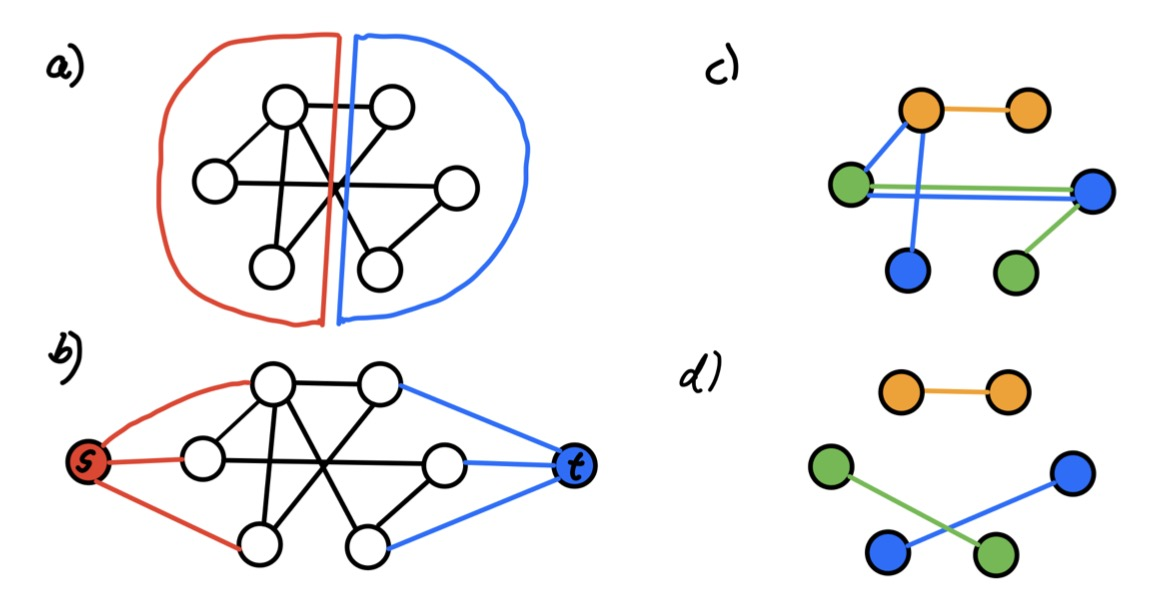
\includegraphics[width=.6\columnwidth]{imgs/cut-match.png}
\end{center}

 In a), a bi-partition $(S_i, \bar{S_i})$ of $V$ is found (requires random walk on $G$). In b), the bi-partition is used to obtain a flow problem where we inject one unit of flow to each vertex in $S_i$ via super-source $s$ and extract one unit of flow from each vertex in $\bar{S_i}$ via super-sink $t$. Every edge is set to have capacity $1/\psi$. Then we solve this problem to get a flow $f$ with $\val(f)=n/2$. If such flow does not exist, then we return the min-cut of this flow problem, removing the dummy source and sink.  c) If such flow exists, we construct a path flow decomposition. For each path, the first vertex is in $S$ and the last vertex in $\bar{S}$. d) We find $M_{i}$ to be the one-to-one matching between endpoints in $S$ and $\bar{S}$ defined by the path flows.

 It can be proven that after $T=\Theta(\log^2 n)$ iterations, the union of the $T$ matchings is a $1/2$-expander and $G$ can be embedded into $H$ with congestion $O(\log^2 n / \psi)$, which certifies that $G$ is a $O(\psi / \log^2 n)$-expander. If one of the iterations presents a cut, then it can be proven that the sparsity of this cut is $O(\psi)$.

\end{multicols*}
\end{document}
